\chapter{Breast Cancer Data Analysis}
A subset of the previously discussed regression methods has been used on gene methylation and expression data from breast cancer patients, aiming to explore how methylation of certain genes affects the expression of others.


\section{Molecular biology background} \label{sec:mol_bio}
This section briefly presents relevant molecular biology mechanisms related to gene expression, discussed thoroughly in \cite{setubal1997introduction}. Each cell in an organism has a number of long DNA molecules, the different sections of which contain information necessary to build specific proteins. These sections of the DNA sequence are called genes and a single gene corresponds to a protein. The beginning of each gene is marked by a promoter, which is a region of the DNA sequence that indicates there is a gene ahead. Recognition of a promoter region initiates the process called transcription, which creates a copy of the gene on an RNA molecule. The produced messenger RNA is then used by the ribosome, a cell structure devoted to protein synthesis.

DNA methylation is a process which attaches methyl groups to parts of the DNA molecule. Methylation changes to the DNA can be inherited by daughter cells in the process of cell division. Consequently, such changes have the ability to dynamically modify the function of the otherwise static DNA sequence throughout the life of an organism. Methylation can occur in the gene body or the promoter region of a gene. In case of the latter, DNA methylation represses the transcription of the gene causing it to no longer be expressed, practically turning off the gene. 


\section{Breast cancer epigenetic dataset}
The publicly available gene methylation and expression data used in this project is provided by the Breast Invasive Carcinoma (TCGA-BRCA \cite{cancer2012comprehensive}) project of The Cancer Genome Atlas (TCGA). Both the gene methylation and expression data is array based and preprocessed to Level 3 in accordance with the TCGA protocols. The contained data is extracted from tissue samples for a subset of 215 patients diagnosed with breast invasive carcinoma available at the time of download, April 2015. 

Illumina Infinium Human DNA Methylation 450 is the platform used for the extraction of the gene methylation data. It quantifies the levels of methylation at specific locations within the genome, denoted as probes. The set of probes is filtered to only retain those with less than $10\%$ missing values across all 215 samples. Each of the retained probes is associated with a specific gene depending on the location of the probe in the genome.

The probes associated with a specific gene are then separated into two subsets depending on their location in the gene sequence - located in the promoter or gene body regions (see Section \ref{sec:mol_bio}). To clarify, probes located in the TSS1500, TSS200, 5'UTR and first exon regions are associated with the promoter region of the gene, while those located in the body or the 3'UTR are mapped to the body region of the gene.

Methylation levels of the promoter and body regions are derived for each gene and patient in the dataset. The methylation level of a gene's promoter region is defined as the mean methylation level of all probes mapped to the gene's promoter region. The methylation level of the gene body is calculated in a similar way, but averaging probes mapped to the body region.

Two datasets are derived through such preprocessing of the initial dataset. One containing the promoter methylation levels for each gene and patient, and another containing the gene body methylation levels for each gene and patient. These two datasets of gene methylation levels, denoted as "Promoter" and "Gene body", provide predictor values for the linear regression modeling performed in the following sections. The former dataset contains data for 468 genes, while the number of predictors in the latter is 479. 

A dataset of gene expression levels is assembled for each of the two methylation datasets from data provided by the TCGA. These datasets contain expression levels for an equivalent set of genes as their corresponding methylation dataset and observations for the same subset of patients.

The choice of epigenetic datasets, their preprocessing and the construction of a gene network, discussed in Section \ref{sec_netwk}, have been carried out prior to the start of my project by Hui Xiao, PhD student in the Computer Laboratory at the University of Cambridge, and Antonella Iuliano, PhD student in the Department of Mathematics at the University of Salerno.

\section{Gene network assembly} \label{sec_netwk}
%\cite{huttenhower2009exploring}
%\cite{zhang2013network}

\section{Regression methods and setup}

\section{Mapping summary}

\pagebreak
%\ref{tab:map_errors}
\begin{table}[H]
	\begin{center}
		\caption{Summary of the mean squared test errors for both datasets}
		\label{tab:map_errors}
		\setlength{\tabcolsep}{18pt}
		\pgfplotstabletypeset[
		multicolumn names,
		col sep=comma,
		header=has colnames,
		display columns/0/.style={string type, column type = {l}},
		display columns/1/.style={string type, column type = {l}},
		display columns/2/.style={column type={S}, string type, column type = {r}},
		display columns/3/.style={column type={S}, column name={$\sigma_{MSE}$}, string type, column type = {r}},
		every head row/.style={
			before row={\toprule}, 
			after row/.add={}{
				\midrule\midrule
			}
		},
		every last row/.style={
			after row=\bottomrule
		},
		every nth row={5}{before row=\midrule},
		]{tables/mapping_errors.csv}
	\end{center}
\end{table}
\begin{figure}[H]
	\centering
	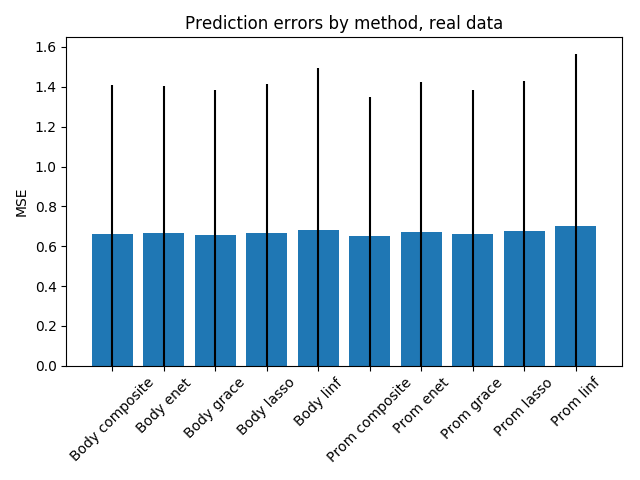
\includegraphics[scale=0.8]{mappings/errors}
	\caption{MSE by regression method and dataset}
	\label{fig:map_errors}
\end{figure}

\pagebreak
%\ref{tab:map_summary}
\begin{table}[H]
	\begin{center}
		\caption{Summary of expression-methylation mappings for both datasets and all considered regression methods; resolved refers to the number of genes with found dependencies to the methylation of others; influencing refers to the number of genes whose methylation affects the expression of others}
		\label{tab:map_summary}
		\pgfplotstabletypeset[
		multicolumn names,
		col sep=comma,
		header=has colnames,
		display columns/0/.style={string type, column type = {l}},
		display columns/1/.style={string type, column type = {l}},
		display columns/2/.style={column type={S}, string type, column type = {|r}},
		display columns/3/.style={column type={S}, string type, column type = {r}},
		display columns/4/.style={column type={S}, string type, column type = {|r}},
		display columns/5/.style={column type={S}, string type, column type = {r}},
		every head row/.style={
			before row={\toprule}, 
			after row/.add={}{
				\midrule\midrule
			}
		},
		every last row/.style={
			after row=\bottomrule
		},
		every nth row={5}{before row=\midrule},
		]{tables/mapping_summary.csv}
	\end{center}
\end{table}
\begin{figure}[H]
	\centering
	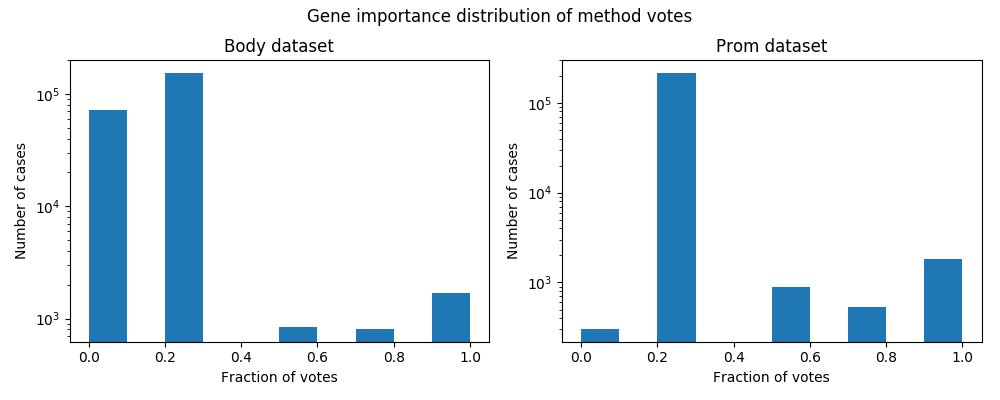
\includegraphics[scale=0.54]{mappings/vote_distribution}
	\caption{Predictor importance fraction of votes distribution for gene body (left) and promoter (right) datasets}
	\label{fig:map_vote_dist}
\end{figure}


\pagebreak
\subsection{Lasso}

\begin{figure}[H]
	\centering
	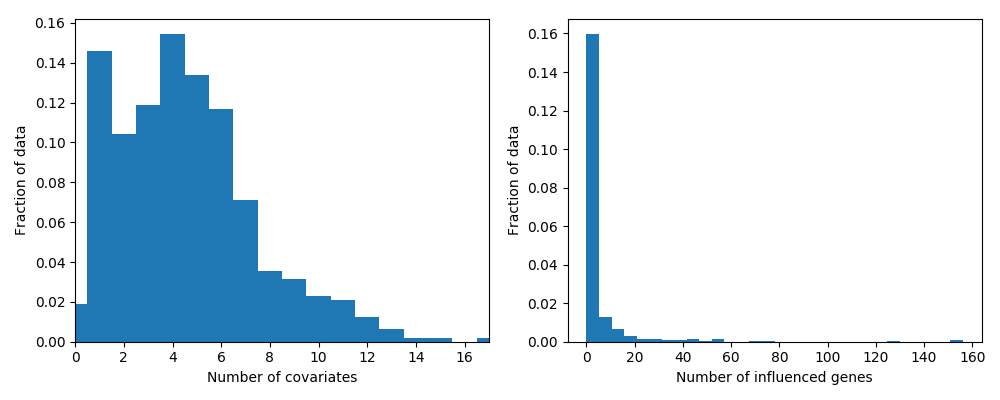
\includegraphics[scale=0.54]{mappings/distributions/Lasso_Body}
	\caption{Lasso mapping dependencies summary for gene body dataset}
	\label{fig:map_body_lasso}
\end{figure}

\begin{figure}[H]
	\centering
	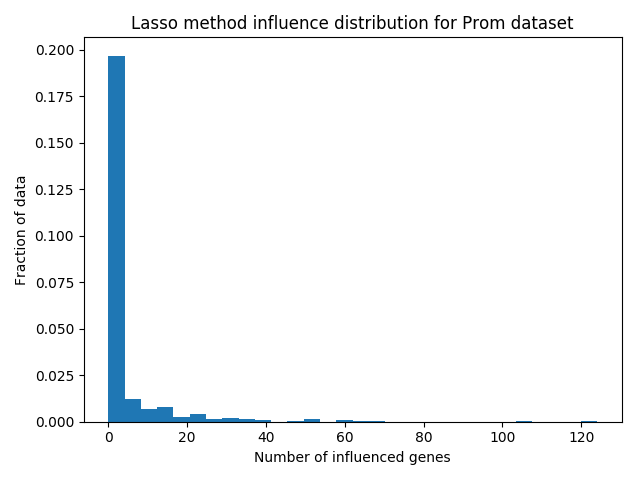
\includegraphics[scale=0.54]{mappings/distributions/Lasso_Prom}
	\caption{Lasso mapping dependencies summary for promoter dataset}
	\label{fig:map_prom_lasso}
\end{figure}


\pagebreak
\subsection{Elastic Net}

\begin{figure}[H]
	\centering
	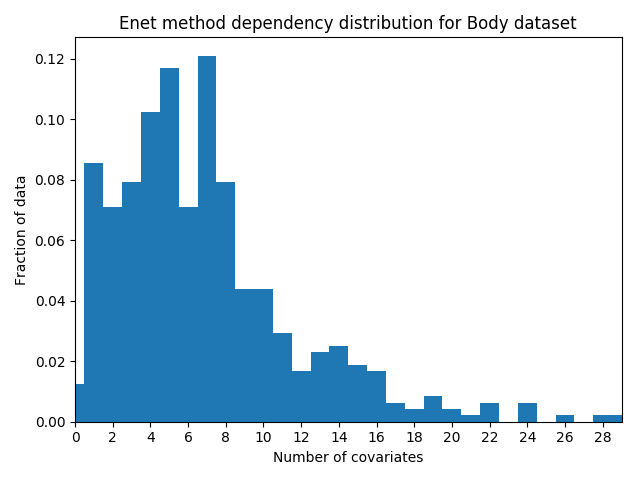
\includegraphics[scale=0.54]{mappings/distributions/Enet_Body}
	\caption{Elastic Net mapping dependencies summary for gene body dataset}
	\label{fig:map_body_enet}
\end{figure}

\begin{figure}[H]
	\centering
	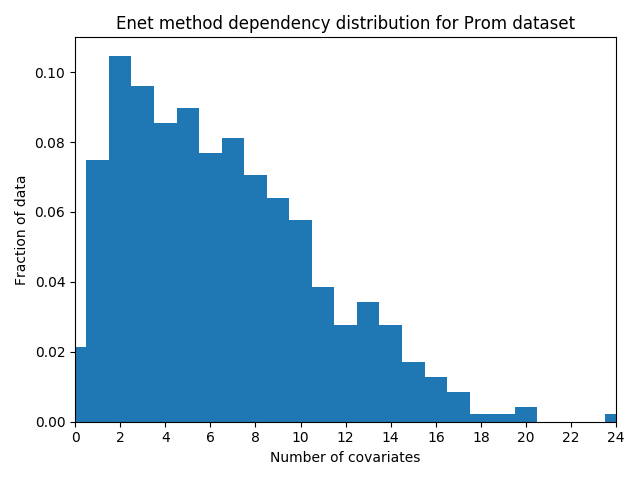
\includegraphics[scale=0.54]{mappings/distributions/Enet_Prom}
	\caption{Elastic Net mapping dependencies summary for promoter dataset}
	\label{fig:map_prom_enet}
\end{figure}


\pagebreak
\subsection{Grace}

\begin{figure}[H]
	\centering
	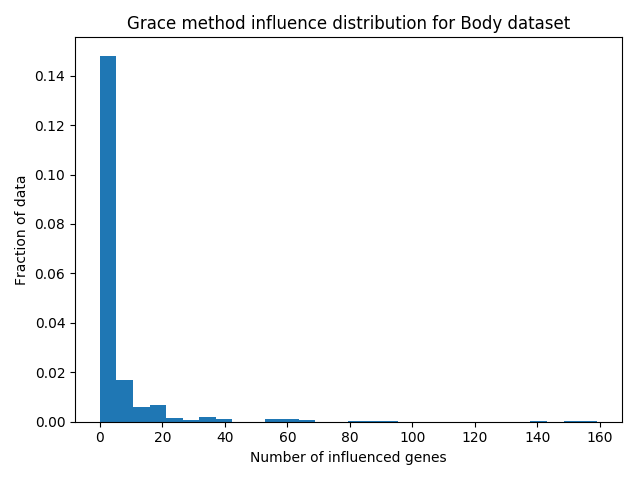
\includegraphics[scale=0.54]{mappings/distributions/Grace_Body}
	\caption{Grace mapping dependencies summary for gene body dataset}
	\label{fig:map_body_grace}
\end{figure}

\begin{figure}[H]
	\centering
	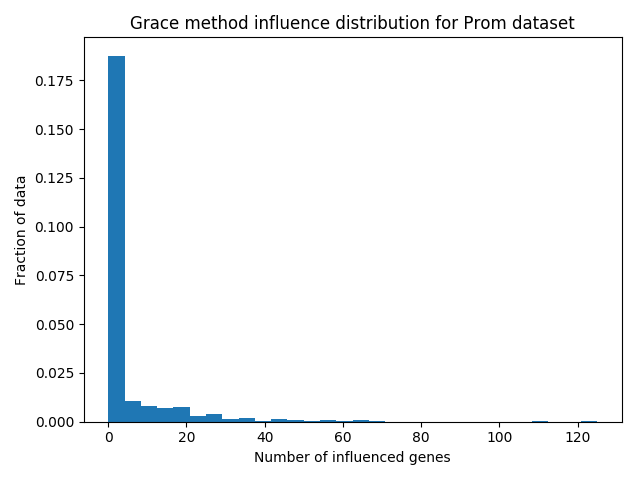
\includegraphics[scale=0.54]{mappings/distributions/Grace_Prom}
	\caption{Grace mapping dependencies summary for promoter dataset}
	\label{fig:map_prom_grace}
\end{figure}


\pagebreak
\subsection{Linf}

\begin{figure}[H]
	\centering
	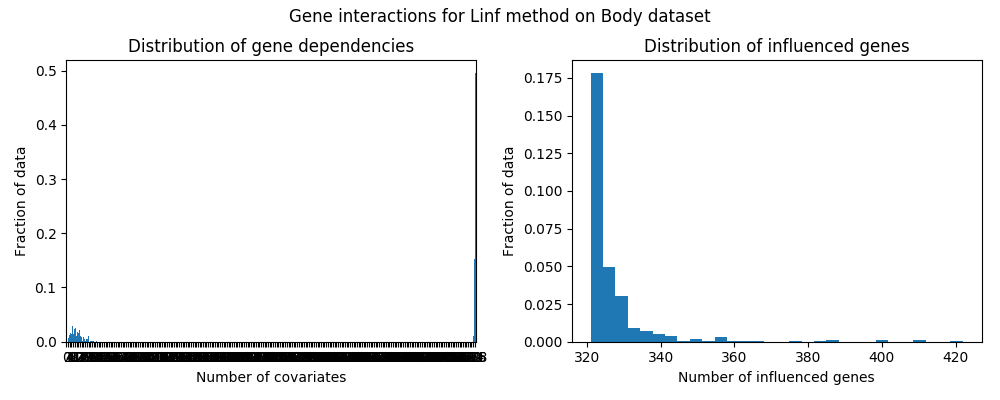
\includegraphics[scale=0.54]{mappings/distributions/Linf_Body}
	\caption{Linf mapping dependencies summary for gene body dataset}
	\label{fig:map_body_linf}
\end{figure}

\begin{figure}[H]
	\centering
	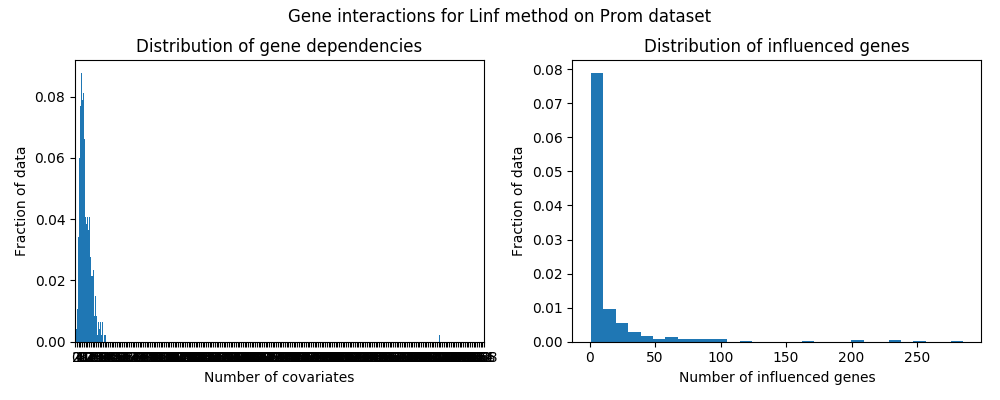
\includegraphics[scale=0.54]{mappings/distributions/Linf_Prom}
	\caption{Linf mapping dependencies summary for promoter dataset}
	\label{fig:map_prom_linf}
\end{figure}


\pagebreak
\subsection{Composite}

\begin{figure}[H]
	\centering
	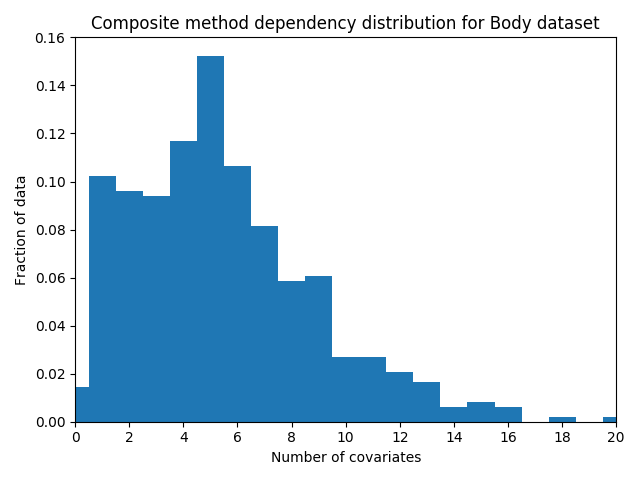
\includegraphics[scale=0.54]{mappings/distributions/Composite_Body}
	\caption{Composite method mapping dependencies summary for gene body dataset}
	\label{fig:map_body_comp}
\end{figure}

\begin{figure}[H]
	\centering
	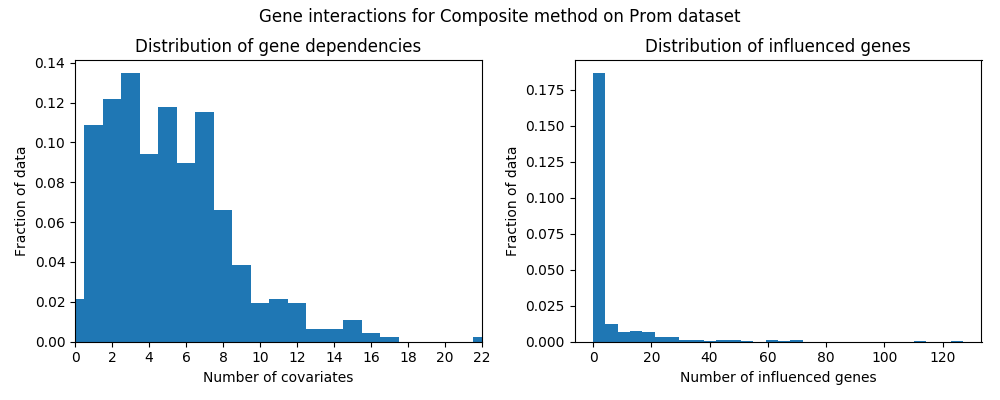
\includegraphics[scale=0.54]{mappings/distributions/Composite_Prom}
	\caption{Composite method mapping dependencies summary for promoter dataset}
	\label{fig:map_prom_comp}
\end{figure}